\documentclass[12pt,a4paper]{article}

% ============================================================
% PACOTES
% ============================================================
\usepackage[utf8]{inputenc}
\usepackage[T1]{fontenc}
\usepackage[brazilian]{babel}
\usepackage{amsmath,amssymb}
\usepackage{graphicx}
\usepackage{booktabs}
\usepackage{caption}
\usepackage{float}
\usepackage{geometry}
\usepackage{hyperref}
\usepackage{xcolor}
\usepackage{enumitem}
\usepackage{array}

\geometry{margin=2.5cm}
\hypersetup{
    colorlinks=true,
    linkcolor=blue,
    citecolor=blue,
    urlcolor=blue
}

% ------------------------------------------------------------
% Ambiente para indicar onde cada figura/imagem deve entrar,
% sem inserir a imagem de fato. Basta trocar o conteúdo do
% \fbox por \includegraphics{caminho/da/imagem.png} depois.
% ------------------------------------------------------------
\newcommand{\figuraPendente}[3]{%
\begin{figure}[H]
    \centering
    \fbox{\begin{minipage}{0.85\textwidth}
        \centering
        \vspace{2.5cm}
        \textbf{[INSERIR FIGURA AQUI]}\\[0.3cm]
        \textit{Arquivo sugerido:} \texttt{#1}\\[0.3cm]
        \textit{Conteúdo:} #2
        \vspace{2.5cm}
    \end{minipage}}
    \caption{#3}
    \label{fig:#1}
\end{figure}
}

% ============================================================
% CABEÇALHO / TÍTULO
% ============================================================
\title{
    \Large \textbf{Avanços em Inteligência Artificial} \\
    \large EELT7025 --- PPGEE, UFPR \\[0.3cm]
    \normalsize Exercícios da Aula 01 \\
    \normalsize Ambiente Computacional, Bibliotecas e Aplicações
}
\author{Adriely Teixeira de Paula, Betina Zynger Capaverde, Emilio Gaudeda Junior}
\date{\today}

% ============================================================
\begin{document}

\maketitle
\tableofcontents
\newpage

% ============================================================
% EXERCÍCIO 1
% ============================================================
\section{Exercício 1 --- Benchmark Iris vs. Wine}

\subsection{Objetivo}
Repetir o benchmark de classificação multiclasse aplicado originalmente ao \emph{Wine Dataset} sobre o \emph{Iris Dataset}, comparando ambos quanto a Accuracy, Precision, Recall, F1-score e tempo de treinamento.

\subsection{Descrição dos datasets}

\begin{table}[H]
\centering
\caption{Características dos datasets utilizados}
\begin{tabular}{lccc}
\toprule
Dataset & Nº de amostras & Nº de atributos & Nº de classes \\
\midrule
Iris  & 150 & 4  & 3 \\
Wine  & 178 & 13 & 3 \\
\bottomrule
\end{tabular}
\end{table}

\subsection{Resultados do benchmark --- Wine}

\begin{table}[H]
\centering
\caption{Benchmark de classificadores --- Wine Dataset (10-fold CV + hold-out 70/30)}
\begin{tabular}{lccccc}
\toprule
Modelo & Acc$_{CV}$ & F1$_{CV}$ & Acc$_{teste}$ & F1$_{teste}$ & T$_{treino}$ (s) \\
\midrule
Logistic Regression & 0.9833 $\pm$ 0.0255 & 0.9829 & 0.9815 & 0.9829 & 0.0120 \\
K-NN (k=5)           & 0.9722 $\pm$ 0.0448 & 0.9729 & 0.9444 & 0.9441 & 0.0018 \\
Decision Tree        & 0.9052 $\pm$ 0.0658 & 0.9076 & 0.9630 & 0.9638 & 0.0047 \\
Random Forest\textsuperscript{*} & 0.9889 & --- & 1.0000 & --- & 1.6077 \\
\bottomrule
\end{tabular}
\\[0.2cm]
\footnotesize{\textsuperscript{*}Melhor modelo geral (maior Acc$_{CV}$ entre os 11 classificadores testados).}
\end{table}

\subsection{Resultados do benchmark --- Iris}

\begin{table}[H]
\centering
\caption{Benchmark de classificadores --- Iris Dataset (10-fold CV + hold-out 70/30)}
\begin{tabular}{lccccc}
\toprule
Modelo & Acc$_{CV}$ & F1$_{CV}$ & Acc$_{teste}$ & F1$_{teste}$ & T$_{treino}$ (s) \\
\midrule
Logistic Regression & 0.9533 $\pm$ 0.0521 & 0.9526 & 0.9111 & 0.9107 & 0.0084 \\
K-NN (k=5)\textsuperscript{*} & 0.9600 $\pm$ 0.0533 & 0.9588 & 0.9111 & 0.9095 & 0.0017 \\
Decision Tree        & 0.9333 $\pm$ 0.0516 & 0.9320 & 0.9111 & 0.9107 & 0.0043 \\
\bottomrule
\end{tabular}
\\[0.2cm]
\footnotesize{\textsuperscript{*}Melhor modelo geral (maior Acc$_{CV}$ entre os 11 classificadores testados).}
\end{table}

\subsection{Tabela comparativa --- resumo dos melhores modelos}

\begin{table}[H]
\centering
\caption{Comparação Iris vs. Wine --- melhor modelo de cada dataset}
\begin{tabular}{lccccc}
\toprule
Dataset & Melhor modelo & Accuracy & Precision & Recall & F1-score \\
\midrule
Iris & K-NN (k=5)      & 0.9111 & 0.9298 & 0.9111 & 0.9095 \\
Wine & Random Forest   & 1.0000 & 1.0000 & 1.0000 & 1.0000 \\
\bottomrule
\end{tabular}
\end{table}

\noindent Accuracy média de CV (todos os modelos): Iris = 0{,}9503; Wine = 0{,}9646.\\
Tempo médio de treinamento (todos os modelos): Iris = 0{,}3503\,s; Wine = 0{,}3659\,s.

\subsection{Figuras}

\begin{figure}[H]
    \centering
    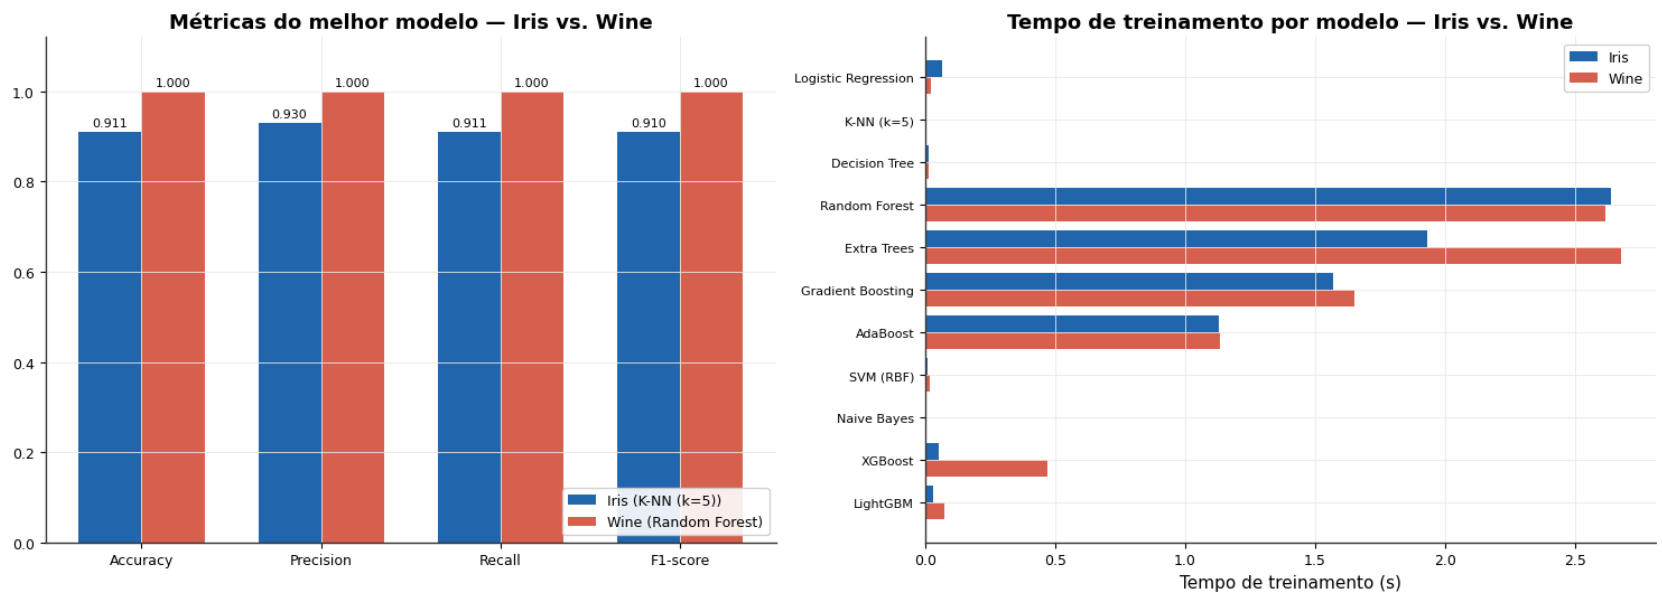
\includegraphics[width=0.85\textwidth]{Figuras_Aula1/fig1-metricas-barras.png}
    \caption{Comparação de métricas principais e tempo de treinamento --- Iris vs. Wine.}
    \label{fig:fig1-metricas-barras}
\end{figure}

\begin{figure}[H]
    \centering
    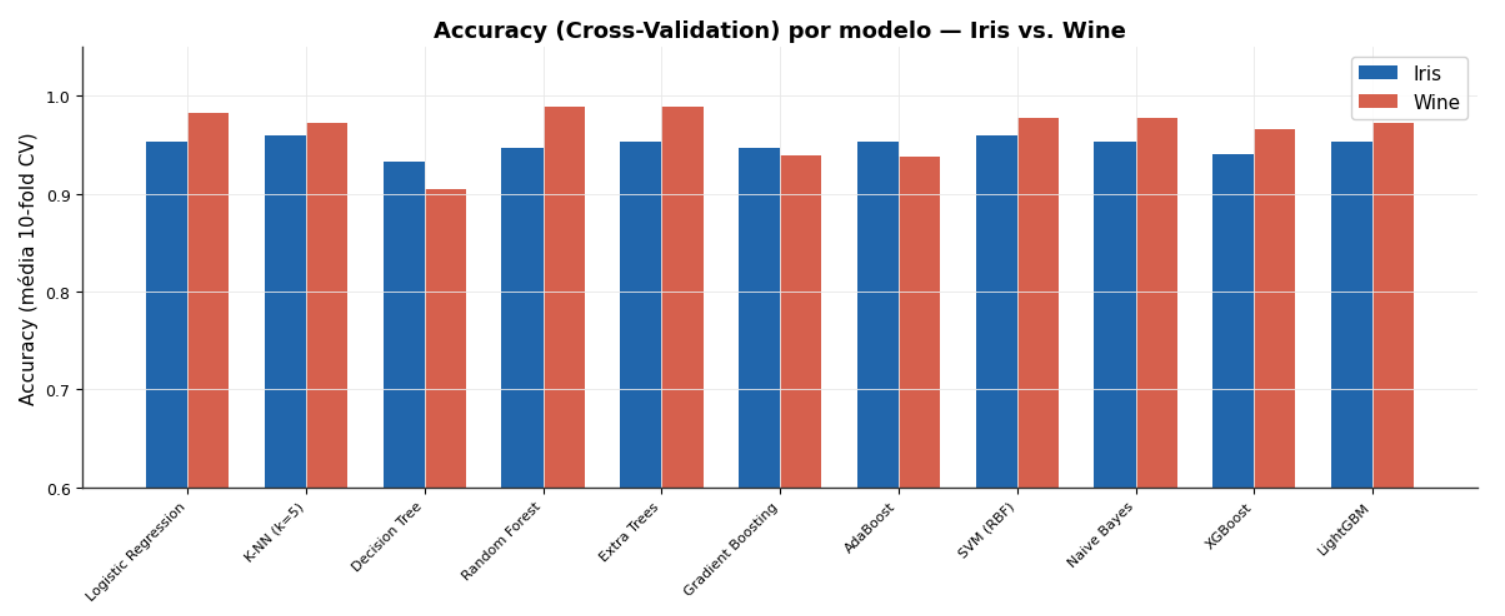
\includegraphics[width=0.85\textwidth]{Figuras_Aula1/fig2-accuracy-cv-modelos.png}
    \caption{Accuracy de Cross-Validation por modelo --- Iris vs. Wine.}
    \label{fig:fig1-metricas-barras}
\end{figure}

\begin{figure}[H]
    \centering
    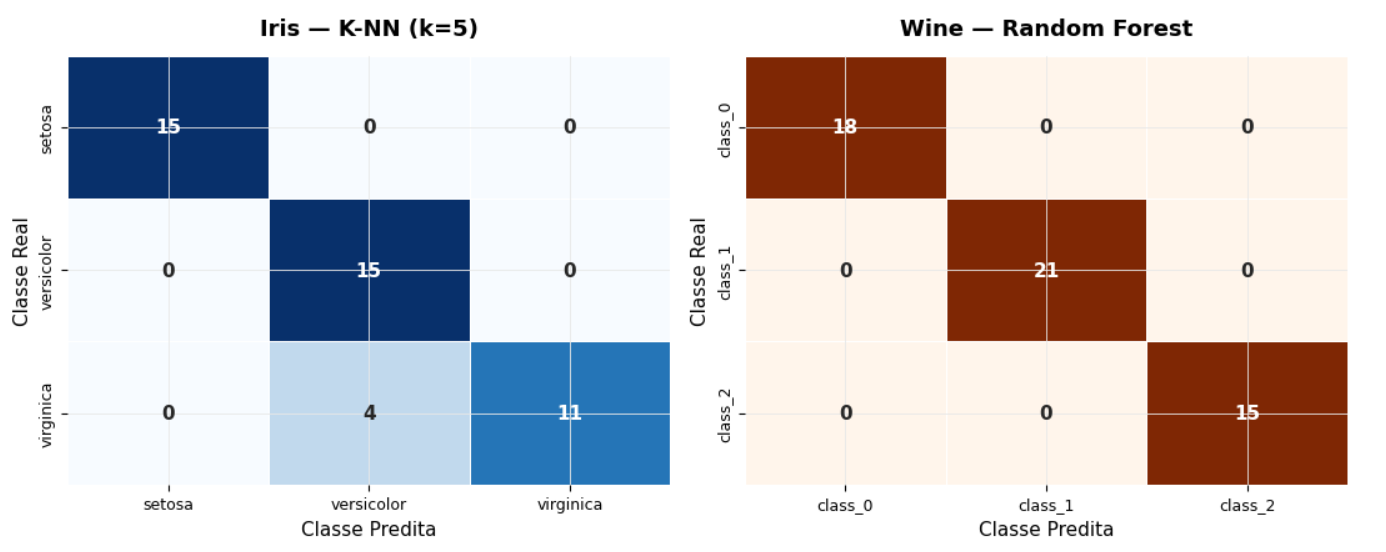
\includegraphics[width=0.85\textwidth]{Figuras_Aula1/fig3-matrizes-confusao.png}
    \caption{Matrizes de confusão dos melhores modelos --- Iris e Wine.}
    \label{fig:fig1-metricas-barras}
\end{figure}


\subsection{Discussão}
O Wine, apesar de ter mais que o triplo de atributos do Iris (13 vs. 4), obteve desempenho de validação cruzada e de teste ligeiramente superior. Isso indica que a quantidade e a qualidade da informação discriminativa contida nos atributos --- e não apenas o número de dimensões ou de classes --- é o fator mais determinante da separabilidade e do desempenho final. O tempo de treinamento, para datasets desse porte, é dominado pela complexidade do algoritmo (ensembles de árvores são consistentemente mais lentos), não pelas diferenças de dimensionalidade entre os dois datasets.

\newpage
% ============================================================
% EXERCÍCIO 2
% ============================================================
\section{Exercício 2 --- Regra 1-SE na Árvore de Decisão (Wine)}

\subsection{Objetivo}
Selecionar, por meio da regra 1-SE (\emph{one standard error rule}), a profundidade (\texttt{max\_depth}) mais simples de uma Árvore de Decisão cuja acurácia média de validação cruzada esteja a no máximo 1 desvio-padrão da melhor acurácia observada.

\subsection{Resultados}

\begin{table}[H]
\centering
\caption{Regra 1-SE --- seleção de \texttt{max\_depth} (Wine, 10-fold CV)}
\begin{tabular}{lccc}
\toprule
Critério & \texttt{max\_depth} & Acc$_{CV}$ (média $\pm$ desvio) & Nº de nós \\
\midrule
Melhor modelo (maior Acc$_{CV}$) & 5 & 0{,}9052 $\pm$ 0{,}0658 & --- \\
Regra 1-SE                        & 2 & 0{,}8542 $\pm$ 0{,}0618 & --- \\
\bottomrule
\end{tabular}
\end{table}

\noindent Limiar 1-SE (melhor média $-$ 1 desvio-padrão) = 0{,}8394.\\
Redução de complexidade: de \texttt{max\_depth}=5 para \texttt{max\_depth}=2 ($-$3 níveis).

\subsection{Figuras}

\begin{figure}[H]
    \centering
    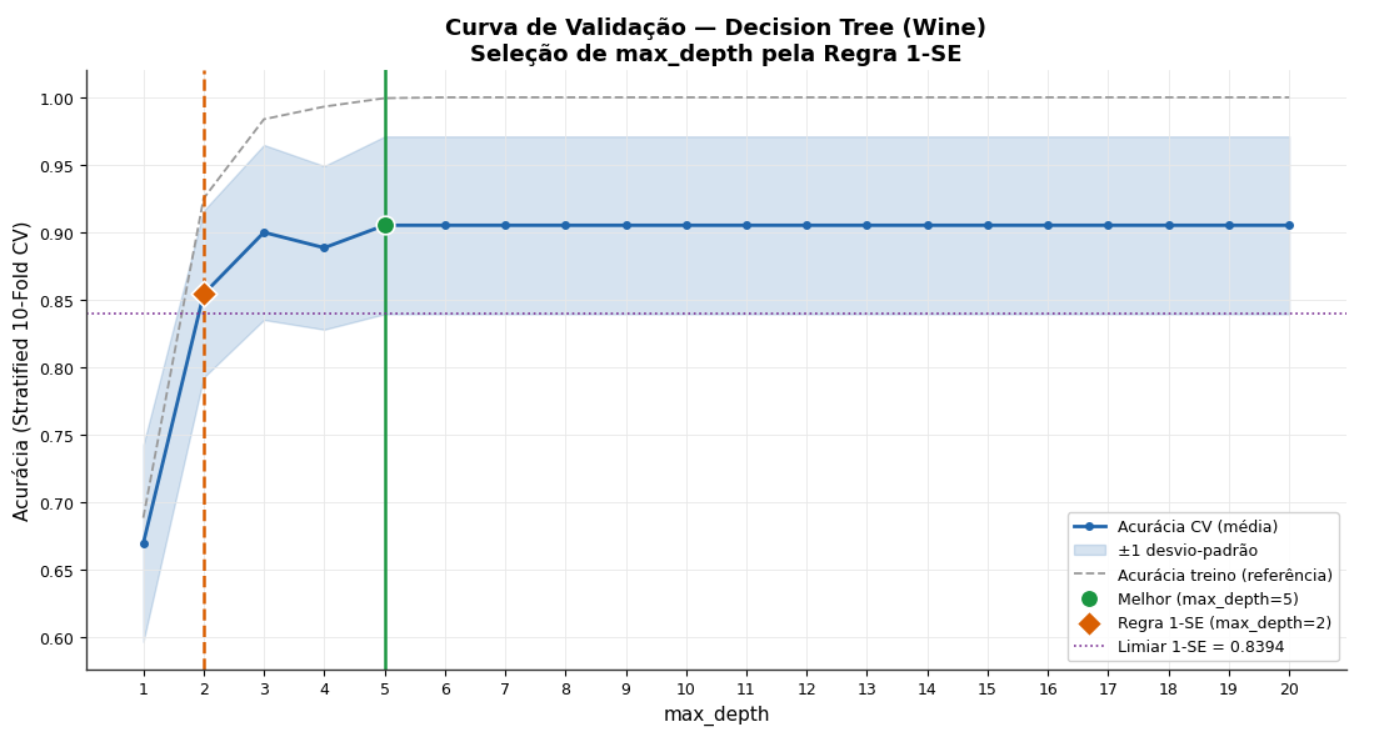
\includegraphics[width=0.85\textwidth]{Figuras_Aula1/fig4-curva-validacao-1se.png}
    \caption{Curva de validação --- seleção de \texttt{max\_depth} pela Regra 1-SE.}
    \label{fig:fig1-metricas-barras}
\end{figure}

\subsection{Discussão}
A árvore mais profunda (\texttt{max\_depth}=5) tende a se ajustar mais ao ruído específico das partições de treino, aumentando a variância do modelo sem ganho estatisticamente relevante de acurácia. A Regra 1-SE parte do princípio de que, se um modelo mais simples atinge acurácia dentro de 1 desvio-padrão do melhor modelo, a diferença observada pode ser atribuída ao ruído da validação cruzada. Assim, escolhe-se a árvore mais rasa (\texttt{max\_depth}=2) que ainda está dentro dessa margem, resultando em um modelo mais simples, mais interpretável e menos propenso a \emph{overfitting}.

\newpage
% ============================================================
% EXERCÍCIO 3
% ============================================================
\section{Exercício 3 --- \texttt{SelectKBest} + \texttt{Ridge} (California Housing)}

\subsection{Objetivo}
Construir um pipeline com seleção automática de atributos (\texttt{SelectKBest} + \texttt{f\_regression}) seguida de regressão \texttt{Ridge}, otimizando conjuntamente $k$ (número de atributos) e $\alpha$ (regularização) via \texttt{GridSearchCV}, e comparar com um \texttt{Ridge} de referência sem seleção de atributos.

\subsection{Dataset}
California Housing: 20.640 amostras, 8 atributos (\texttt{MedInc}, \texttt{HouseAge}, \texttt{AveRooms}, \texttt{AveBedrms}, \texttt{Population}, \texttt{AveOccup}, \texttt{Latitude}, \texttt{Longitude}), variável-alvo \texttt{MedHouseVal} (valor mediano das casas, em US\$100.000).

\subsection{Melhores hiperparâmetros}

\begin{table}[H]
\centering
\caption{Melhores hiperparâmetros --- \texttt{GridSearchCV} (10-fold)}
\begin{tabular}{lccc}
\toprule
Pipeline & $k$ (nº atributos) & $\alpha$ (Ridge) & RMSE (CV, treino) \\
\midrule
SelectKBest + Ridge & 8 & 3{,}162 & 0{,}7205 \\
Ridge (referência)  & 8 & 3{,}162 & 0{,}7205 \\
\bottomrule
\end{tabular}
\end{table}

\noindent \textit{Observação:} o \texttt{GridSearchCV} selecionou $k=8$ (todos os atributos disponíveis), portanto, neste caso, o pipeline \texttt{SelectKBest+Ridge} converge para o mesmo modelo do \texttt{Ridge} de referência.

\subsection{Métricas de desempenho}

\begin{table}[H]
\centering
\caption{RMSE, MAE e R² --- treino vs. teste}
\begin{tabular}{lcccccc}
\toprule
Modelo & RMSE$_{tr}$ & MAE$_{tr}$ & R\textsuperscript{2}$_{tr}$ & RMSE$_{te}$ & MAE$_{te}$ & R\textsuperscript{2}$_{te}$ \\
\midrule
SelectKBest + Ridge & 0{,}7197 & 0{,}5286 & 0{,}6126 & 0{,}8513 & 0{,}5541 & 0{,}4470 \\
Ridge (referência)  & 0{,}7197 & 0{,}5286 & 0{,}6126 & 0{,}8513 & 0{,}5541 & 0{,}4470 \\
\bottomrule
\end{tabular}
\end{table}

\subsection{Figuras}

\begin{figure}[H]
    \centering
    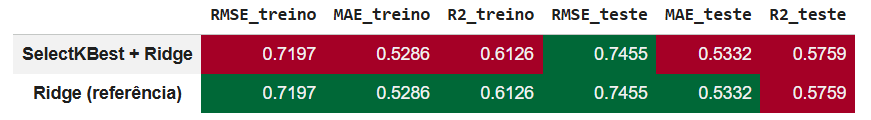
\includegraphics[width=0.85\textwidth]{Figuras_Aula1/fig5-scores-selectkbest.png}
    \caption{Importância dos atributos (\texttt{SelectKBest}) --- California Housing.}
    \label{fig:fig1-metricas-barras}
\end{figure}

\begin{figure}[H]
    \centering
    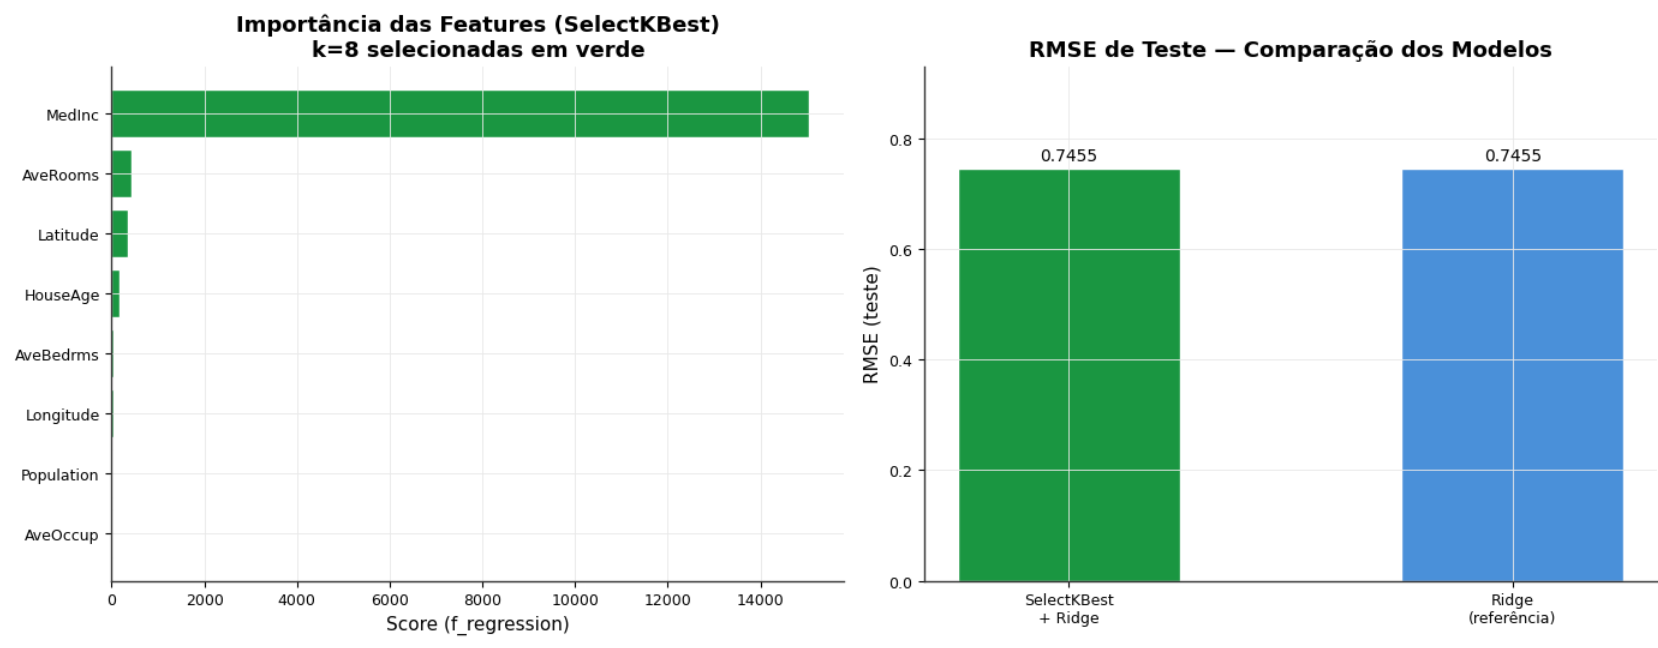
\includegraphics[width=0.85\textwidth]{Figuras_Aula1/fig6-rmse-comparacao.png}
    \caption{RMSE de teste --- comparação dos dois modelos.}
    \label{fig:fig1-metricas-barras}
\end{figure}


\subsection{Discussão}
Como o \texttt{GridSearchCV} selecionou todos os 8 atributos, não houve redução de dimensionalidade neste caso -- praticamente todos os atributos do California Housing carregam alguma informação relevante sobre o preço mediano dos imóveis, sem um subconjunto pequeno claramente dominante em poder preditivo. Ainda assim, o \texttt{SelectKBest} continua sendo uma ferramenta útil em datasets com mais atributos redundantes/irrelevantes, situação em que reduziria a complexidade do modelo com perda mínima de desempenho.

\newpage
% ============================================================
% EXERCÍCIO 4
% ============================================================
\section{Exercício 4 --- Bootstrap para Incerteza do AUC-ROC (Breast Cancer)}

\subsection{Objetivo}
Estimar o AUC-ROC médio e o intervalo de confiança de 95\% de cada classificador por meio de 1000 reamostragens \emph{Bootstrap} do conjunto de teste, mantendo o modelo fixo (treinado uma única vez).

\subsection{Dataset}
Breast Cancer Wisconsin: 569 amostras, 30 atributos, 2 classes (212 malignos, 357 benignos).

\subsection{Resultados --- AUC-ROC com IC 95\% (Bootstrap, 1000 reamostragens)}

\begin{table}[H]
\centering
\caption{AUC-ROC médio e intervalo de confiança de 95\% por classificador}
\begin{tabular}{lccc}
\toprule
Modelo & AUC médio & IC 95\% & Largura do IC \\
\midrule
Logistic Regression\textsuperscript{*} & 0{,}9978 & [0{,}9916, 1{,}0000] & 0{,}0084 \\
SVM (RBF)            & 0{,}9969 & [0{,}9894, 1{,}0000] & 0{,}0106 \\
Random Forest        & 0{,}9948 & [0{,}9869, 0{,}9993] & 0{,}0124 \\
XGBoost              & 0{,}9937 & [0{,}9840, 0{,}9998] & 0{,}0158 \\
Gradient Boosting    & 0{,}9924 & [0{,}9820, 0{,}9986] & 0{,}0167 \\
LightGBM             & 0{,}9889 & [0{,}9723, 0{,}9996] & 0{,}0273 \\
K-NN (k=5)           & 0{,}9846 & [0{,}9547, 1{,}0000] & 0{,}0453 \\
Decision Tree        & 0{,}9182 & [0{,}8571, 0{,}9706] & 0{,}1135 \\
\bottomrule
\end{tabular}
\\[0.2cm]
\footnotesize{\textsuperscript{*}Maior AUC médio entre os 8 classificadores testados.}
\end{table}

\subsection{Figuras}

\begin{figure}[H]
    \centering
    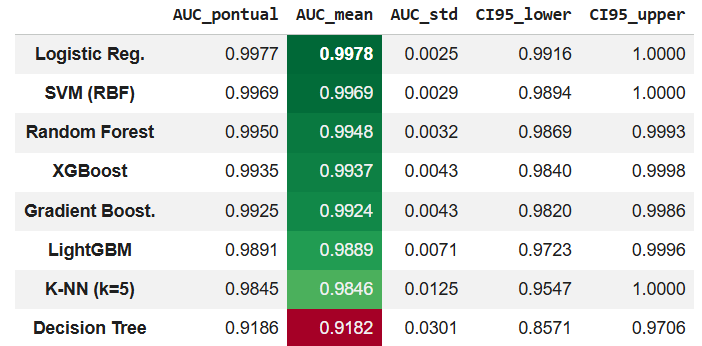
\includegraphics[width=0.85\textwidth]{Figuras_Aula1/fig7-auc-ic95-barras.png}
    \caption{AUC-ROC médio $\pm$ IC 95\% --- Bootstrap, 1000 reamostragens.}
    \label{fig:fig1-metricas-barras}
\end{figure}

\begin{figure}[H]
    \centering
    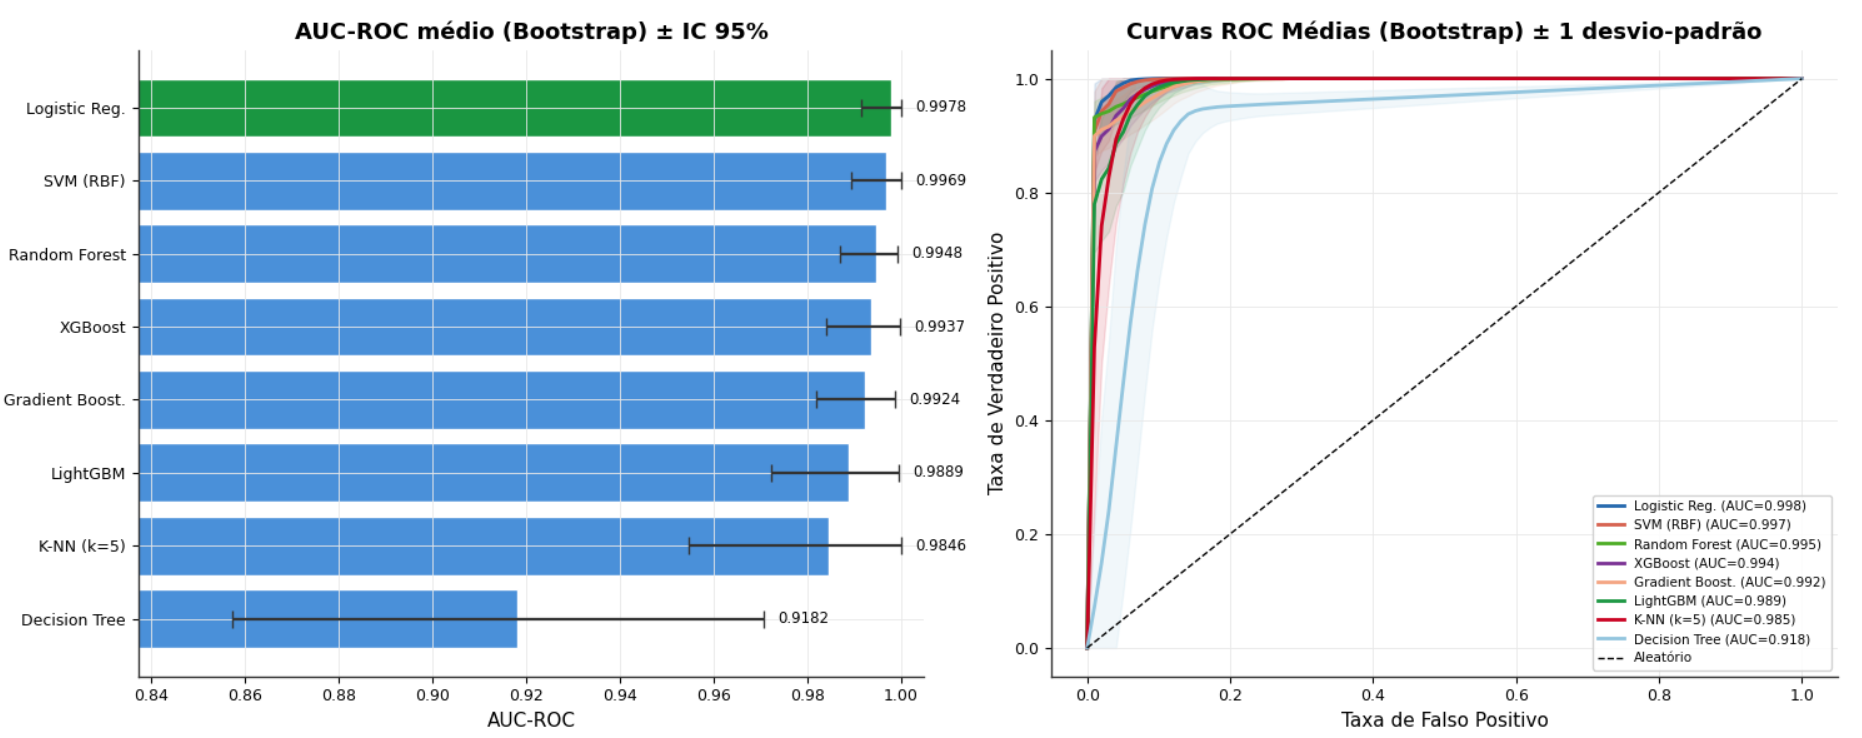
\includegraphics[width=0.85\textwidth]{Figuras_Aula1/fig8-curvas-roc-medias.png}
    \caption{Curvas ROC médias com banda de incerteza --- Breast Cancer.}
    \label{fig:fig1-metricas-barras}
\end{figure}


\subsection{Sobreposição dos intervalos de confiança}
Todos os modelos, exceto a Decision Tree, apresentam IC 95\% sobreposto ao do melhor modelo (Logistic Regression) --- ou seja, \textbf{não há evidência estatística suficiente, a 95\% de confiança, de que a Logistic Regression seja de fato superior} a SVM, Random Forest, XGBoost, Gradient Boosting, LightGBM ou K-NN neste dataset. Apenas a Decision Tree (AUC=0{,}9182, IC=[0{,}8571; 0{,}9706]) apresenta IC claramente disjunto do melhor modelo, indicando desempenho genuinamente inferior.

\subsection{Discussão}
O Breast Cancer Wisconsin é um dataset de alta separabilidade, de modo que mesmo modelos simples (Logistic Regression) atingem AUC muito próximo de modelos mais complexos. A ampla sobreposição dos intervalos de confiança reforça que escolher o modelo ``vencedor'' apenas pelo maior AUC pontual pode ser enganoso; quando os IC se sobrepõem, é mais robusto considerar outros critérios de decisão (tempo de treinamento/inferência, interpretabilidade, robustez), reservando a comparação estrita de AUC para os casos em que os intervalos são claramente disjuntos --- como ocorre aqui apenas com a Decision Tree.

\newpage
% ============================================================
% CONCLUSÃO GERAL
% ============================================================
\section{Considerações Finais}

Os quatro exercícios ilustram, em conjunto, boas práticas centrais em aprendizado de máquina: (i) comparar modelos de forma justa exige as mesmas métricas e o mesmo protocolo de validação (Exercício 1); (ii) a seleção de hiperparâmetros não deve se basear apenas no ponto de máxima performance média, mas considerar a incerteza da estimativa (Exercício 2, regra 1-SE); (iii) pipelines de seleção de atributos devem ser validados com a mesma rigor de otimização de hiperparâmetros que os demais componentes do modelo (Exercício 3); e (iv) toda métrica pontual de desempenho carrega incerteza amostral, que deve ser quantificada (por exemplo, via Bootstrap) antes de declarar um modelo superior a outro (Exercício 4).

\end{document}